\section{Teaser}

% \teaser{
% 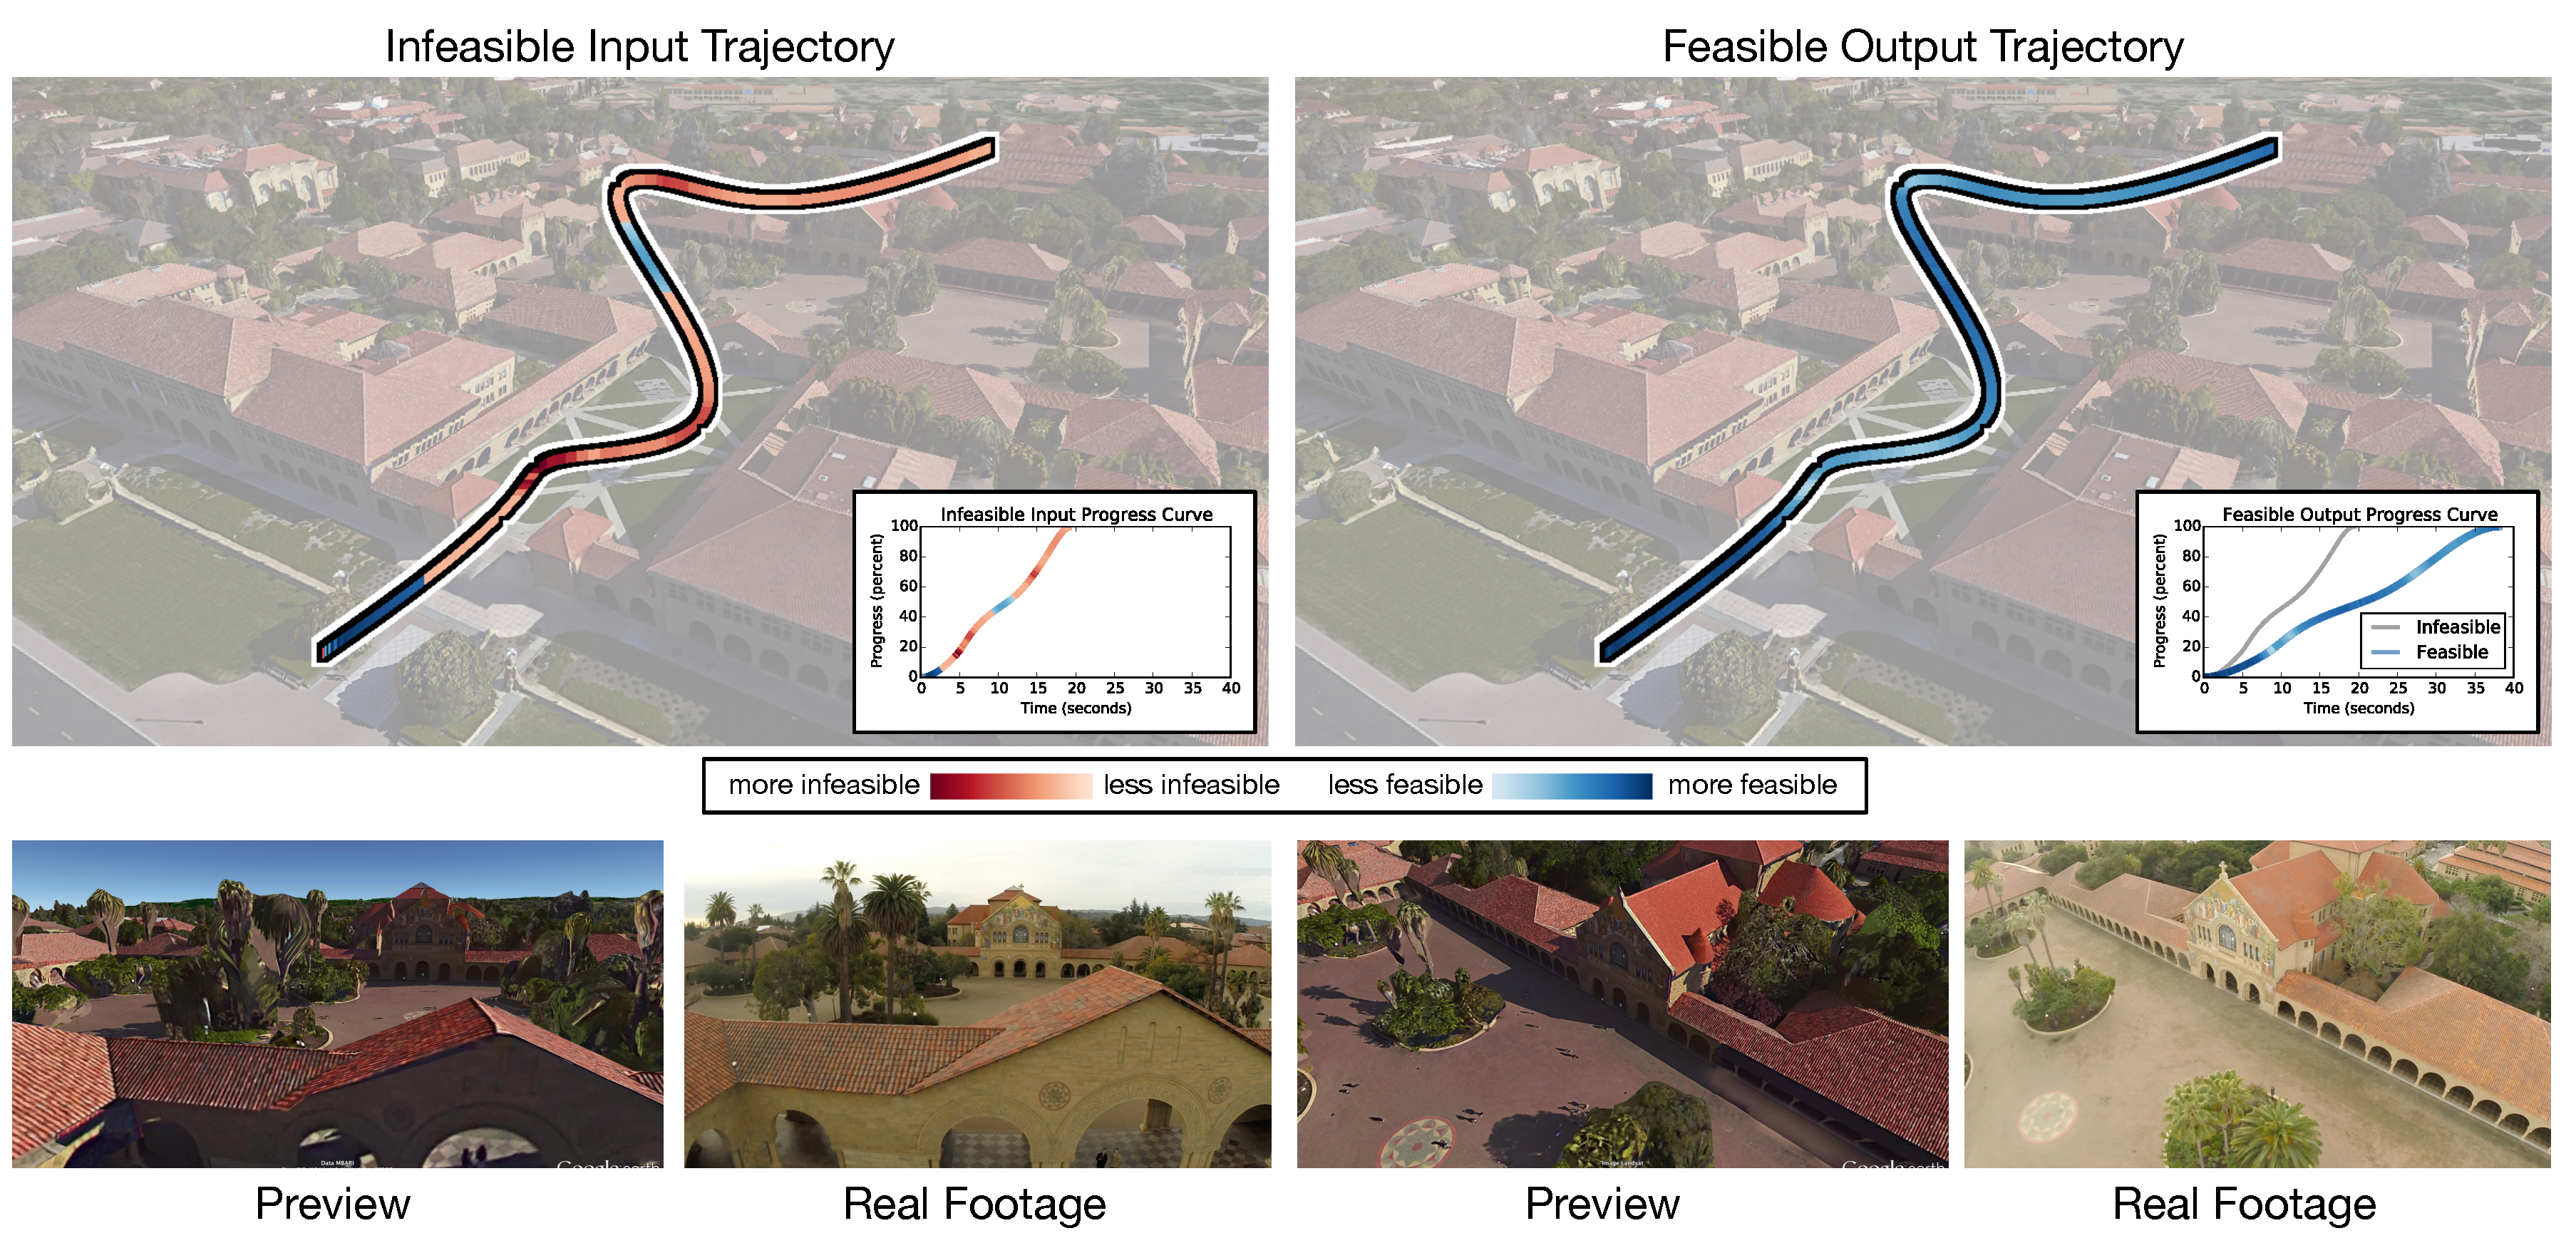
\includegraphics[width=7.0in]{images/06_teaser.pdf}
% \caption{
% Our algorithm for generating feasible quadrotor camera trajectories.
% Our algorithm takes as input a infeasible quadrotor camera trajectory (top row, left) and produces as output a feasible trajectory that is as similar as possible to the input trajectory (top row, right).
% By design, our algorithm does not change the spatial layout or  visual contents of the input trajectory.
% Instead, our algorithm guarantees the feasibility of the output trajectory by re-timing the input trajectory, perturbing its timing as little as possible while remaining within velocity and control force limits (top row, insets).
% Our algorithm runs at interactive rates, solving for the feasible trajectory shown above in less than 2 seconds.
% Infeasible trajectories can be unsafe to fly on real quadrotor cameras, but we can safely fly the feasible trajectories generated by our algorithm, producing real video footage that is faithful to a \textsc{Google Earth} shot preview (bottom row).
% }
% \label{fig:teaser}
% }
